%%% LaTeX Template
%%% This template is made for project reports
%%%	You may adjust it to your own needs/purposes
%%%
%%% Copyright: http://www.howtotex.com/
%%% Date: March 2011

%%% Preamble
\documentclass[paper=a4, fontsize=11pt]{scrartcl}	% Article class of KOMA-script with 11pt font and a4 format
\usepackage[T1]{fontenc}
\usepackage{fourier}

\usepackage[english]{babel}							% English language/hyphenation
\usepackage[protrusion=true,expansion=true]{microtype}	% Better typography
\usepackage{amsmath,amsfonts,amsthm}				% Math packages
\usepackage[pdftex]{graphicx}							% Enable pdflatex
\usepackage{url}
\usepackage{algorithm}
\usepackage{algorithmic}
\usepackage{amsthm}

\usepackage{graphicx} 

    %%% Custom sectioning (sectsty package)
\usepackage{sectsty}						% Custom sectioning (see below)
\allsectionsfont{\centering \normalfont\scshape}	% Change font of al section commands


%%% Custom headers/footers (fancyhdr package)
\usepackage{fancyhdr}
\pagestyle{fancyplain}
\fancyhead{}								% No page header
%fancyfoot[L]{\small \url{HowToTeX.com}}		% You may remove/edit this line 
%\fancyfoot[C]{}							% Empty
\fancyfoot[C]{\thepage}						% Pagenumbering
\renewcommand{\headrulewidth}{0pt}			% Remove header underlines
\renewcommand{\footrulewidth}{0pt}			% Remove footer underlines
\setlength{\headheight}{13.6pt}


%%% Equation and float numbering
\numberwithin{equation}{section}		% Equationnumbering: section.eq#
\numberwithin{figure}{section}		% Figurenumbering: section.fig#
\numberwithin{table}{section}		% Tablenumbering: section.tab#


%%% Maketitle metadata
\newcommand{\horrule}[1]{\rule{\linewidth}{#1}} 	% Horizontal rule
\newtheorem{theorem}{Theorem}[section]
\newtheorem{lemma}[theorem]{Lemma}
\newtheorem{proposition}[theorem]{Proposition}
\newtheorem{corollary}[theorem]{Corollary}

\title{
    %\vspace{-1in} 	
    \usefont{OT1}{bch}{b}{n}
    \normalfont \normalsize \textsc{CS 6150 - Advanced Algorithms\\
    Fall 2011\\
    School of Computing\\ 
    University of Utah} \\ [25pt]
    \horrule{0.5pt} \\[0.4cm]
    \huge Primality Testing \\
    \horrule{2pt} \\[0.5cm]
}
\author{
    \normalfont \normalsize Arijit Banerjee, Suchit Maindola, Srikanth Manikarnike\\
    [-3pt] \normalsize \today
}
\date{}


%%% Begin document
\begin{document}
\bibliographystyle{plain}
\maketitle
\section{Problem Statement}
\paragraph{}The aim of this project is to implement a very widely studied problem of Mathematics -- primality testing -- as efficiently as possible. In saying so, our main focus is to successfully implement a breakthrough achieved in 2002 by Agrawal, Kayal and Saxena (AKS)[1][2] who came up with the "first published primality-proving algorithm to be simultaneously general, polynomial, deterministic and unconditional". Although, this is a worst-case polynomial time algorithm that works on any general number deterministically and is not dependent on yet unproven hypothesis, it does not necessarily give the best running time for all possible inputs. There are other non-determinisitic, approximate, polynomial time algorithms like the Miller Rabin test, the Lucas-Lehmer test for Mersenne numbers and Pepin's test but these algorithms are "constrained" in some way or the other.

\section{Motivation}
\paragraph{} Prime numbers are used extensively in a broad spectrum of fields. 
\begin{itemize}
\item \textbf{Public Key Cryptography\\}
With a pair $public$ and $private$ keys generated using prime numbers, cryptographic algorithms generate cipher text from plain text and vice versa.
\[Plain text = (Cypher text^e) \mod k\]
where, $e$ is a product of two large primes $p$ and  $q$ and $k$ is the public key.
\item \textbf{Modular Arithmetic}\\
Hash functions are a good example of use of prime numbers for modular arithmetic. 
\[h_{a,b}(x)=[(ax+b) \mod n] \mod k \]
where, $n$ is a prime number
\item \textbf{Pattern Recognition}\\
Finger printing words of an alphabet, used in pattern recognition,  can be done using prime numbers. For an alphabet $A = \{x_0, .., x_m\}$, $p_i$, the $i^{th}$ prime greater than $m$ is generated. Using weighted averages $\forall x_i \in A, w_i = x_i/p_i$, fast finger-printing can be performed [3].
\item \textbf{Pseudo Random Number Generation}\\
Recurrence of the form:
\[Z_k+1 = (a \cdot Z_k + r) \mod k \]
where, $r$ and $k$ are relatively prime, known as Linear Congruential Generator Algorithm is used to generate pseudo random numbers. 
\end{itemize}

\section{Literature Review}
\paragraph{}A natural number is said to a prime number if it is greater than one and has no other divisors other than 1 and itself. [4] Though widely studied, it took about 2300 years to come up with a deterministic polynomial time algorithm. While it was always believed that one could produce a polynomial deterministic algorithm, "one reason for the excitement within the mathematical community is not only does this algorithm settle a long-standing problem, it also does so in a brilliantly simple manner. Everyone is now wondering what else has been similarly overlooked".[5]

\paragraph{} Existing algorithms to test for primality of a number can be categorized as probabilistic and deterministic. While probabilistic algorithms could result in false positives i.e., determining a composite number as prime, they do not produce false negatives i.e., determining a prime number as composite. The probability of a false positive is quite small for numbers that are not very large. Deterministic algorithms, however, compute the primality or compositeness of a number correctly every time.\\

\subsection{Characteristics of Primality Testing Algorithms}
%\begin{itemize}
\paragraph {Specificity vs. Generality}
There exist extremely fast primality tests such as - the Lucas--Lehmer test for Mersenne numbers, and Pepin's test for Fermat's number. Though fast, these tests are specific for a small subset of numbers. Although these algorithms could be used in our implementation, a general primality testing algorithm is needed to handle any number $\in N$.

\paragraph{ Probabilistic vs. Deterministic}
Deterministic algorithms such as cyclotomy test have a running time that can be proven to be $O((\log n)^{c\log \log \log n})$. [8] Determinism is a necessary characteristic for a primality testing algorithm. Nonetheless, probabilistic algorithm are so much faster than deterministic ones that, one often finds himself incorporating a probabilistic algorithms in his primality tester. Low probability of false negatives, zero false positives and ability to repeat the test for a given input are some of the reasons why. Some tests that we considered were Miller--Rabin primality test, Solovay--Strassen primality test. 

\paragraph{Polynomial vs. Non-polynomial}
The choice between a polynomial algorithm over a non-polynomial algorithm, though glaringly obvious, needs significant consideration. An algorithm with a polynomial running time is one whose running time can be expressed a polynomial of the length of the input, and hence the number bits in it. This however, does not mean they are the fastest solutions around. Non-polynomial algorithms, such as Fermat's Theorem, is deterministic but this test requires a partial factorization of $n - 1$ the running time is still quite slow in the worst case. Faster algorithms like the probabilistic Miller-Rabin Test runs in polynomial time over all inputs, but its correctness depends on the truth of the yet unproven generalization of the Reimann hypothesis. [6] And lastly the AKS algorithm - both polynomial and deterministic can be painfully slow for smaller inputs.[8]

\paragraph{}Our choice of algorithms to implement the fastest primality tester for this course project must be able to find a sweet spot between determinism, polynomial run time and speed for smaller inputs that polynomial algorithms take too long to process. We will discuss our approach in detail in the Implementation section. 
%\end{itemize}

\subsection{Existing Primality Testing Algorithms}
\paragraph{}Abundant and continuous research is being conducted to analyze the unique characteristic of natural numbers - primality. Based on the application, prime number generators target speed, correctness and polynomial runtime. We describe the following algorithms and our choices in this section.

\subsubsection{Sieve of Eratosthenes - A Na\"{i}ve Approach}
\paragraph{}Named after the ancient Greek mathematician, Eratosthenes of Cyrene, this algorithm is claimed to be the oldest known algorithm to generate prime numbers, originating around 220 B.C. E. The sieve literally "sieves out" every second number after two -- the smallest prime -- (or multiples of two), then moves to the next available (3) and continues to "sieve out" every multiple of 3 and so on. This algorithm is still important today in number research theory [9] and is found to be the most efficient method to find all small primes (less than 10 million) [10]. 

\begin{algorithm}
\caption{Sieve of Eratosthenes}
\label{alg1}
\begin{algorithmic}[1]
\STATE Create a list of consecutive integers from 2 to $n: (2, 3, 4, .... , n)$.
\STATE $p \leftarrow 2$
\STATE Compute integral multiples of $p$ and mark every number strictly greater than $p$ in the list.
\STATE Find the first number greater than $p$ in the list that is not marked
\STATE Let $p$ equal this number (the next prime).
\STATE If there are no more numbers marked in the list, stop. Else, repeat step 3.
\end{algorithmic}
\end{algorithm}

\paragraph{}

\subsubsection{Fermat's Theorem - The Elegant}
\paragraph{}Pierre de Fermat stated his theorem on October 18, 1640, as 
\["p \text{ divides } a^{p-1}-1 \text{ whenever }p\text{ is prime and }a\text{ is coprime to }p"\]
\paragraph{}This algorithm so elegantly states a fact of number theory. This special property stated by Fermat was a stepping stone for researchers around the world to produce a polynomial time algorithm for primality testing.[11] Mathematically, Fermat's theorem can be written as,
\[a^p \equiv 1 \mod p\]
\paragraph{}Using this hypothesis, we can modify the Sieve of Eratosthenes and reduce its running time to a mere polynomial of the input $n$.
\begin{algorithm}
\caption{Fermat's Test}
\label{alg2}
\begin{algorithmic}[1]
\FOR{$i = 2$ to $n$}
\IF {$n$ is of the form $i^n \equiv 1\mod n$}
\RETURN false
\ENDIF
\ENDFOR
\RETURN true
\end{algorithmic}
\end{algorithm}

\paragraph{}As with any theorem, there are exceptions. In 1910, Robert Carmichael found the first smallest number 561 that doesn't obey this rule. He went on define these numbers as "a composite positive integer $n$ which satisfies the congruence
\[b^{n-1} \equiv 1 \mod n\]
for all integers $b$ which are relatively prime to $n$[12]. These numbers are pseudo-prime or probably-prime [13] and are known as Carmichael Numbers. 

\subsubsection{Miller-Rabin Algorithm - Mr. Flash}
\paragraph{}Miller--Rabin primality test is an algorithm which determines whether a given number is prime deterministically. Its determinism, however relies on the unproven generalized Riemann hypothesis (GRH). The original version proposed by Gary L. Miller, in 1975, is  deterministic based on GRH. Michael O. Rabin modified it to obtain an unconditional probabilistic algorithm.

\paragraph{}The Miller--Rabin test is based on the claim that if we can find an $a$ such that
\[a^d \not\equiv 1 \mod n\] and
\[a^{2^rd} \not\equiv -1 \mod n \text{	 for all } 0 \leq r \leq s-1\]
then $n$ is not prime. The algorithm for Miller-Rabin Test is given below.
\begin{algorithm}
\caption{Miller-Rabin Test}
\label{alg3}
\begin{algorithmic}[-3]
\STATE \textbf{Input:} n $>$ 3, an odd integer to be tested for primality;
\STATE \textbf{Input:} $k$, a parameter that determines the accuracy of the test
\STATE \textbf{Output:} composite if $n$ is composite, otherwise probably prime
\STATE write $n -1$ as $2^s\cdot d$ with $d$ odd by factoring powers of 2 from $n-1$
\LOOP
\STATE repeat $k$ times
\STATE pick a random integer $a$ in the range $[4, n-2]$
\STATE $x \leftarrow a^d \mod n$
\IF {$x = 1$ or $x = n -1$} 
\STATE do next \textbf{loop}
\ENDIF
\FOR{$r = 1$ to $s-1$}
\STATE $x \leftarrow x^2 \mod n$
\IF{ $x=1$}
\RETURN COMPOSITE
\ENDIF
\IF {$x = n-1$}
\STATE do next \textbf{loop}
\ENDIF
\ENDFOR
\RETURN COMPOSITE
\ENDLOOP
\RETURN PROBABLY PRIME
\end{algorithmic}
\end{algorithm}
\paragraph{}The running time of this algorithm is $O(k \log^3n)$, where $k$ is the number of different values of $a$ we test; hence this is an efficient, polynomial-time algorithm. The probability of getting a correct result improves with the number of bases $a$ we test with. For any odd composite $n$, at least $\frac{3}{4}$ of the bases $a$ are witnesses for the compositeness of $n$. If $n$ is composite, then the Miller-Rabin test declares $n$ probably prime with at most $4^{-k} $ probability[6]. The error bound of Miller-Rabin is $4^{-1} = 25 \%$ in the worst case.The probability of a false negative of Solovay-Strassen test is $2^{-k}$ and hence its error bound is $\frac{1}{2}.$ \\

%\begin {itemize}
\paragraph{Deterministic Variant of Miller-Rabin Test}
Miller-Rabin can be made deterministic by trying all possible $a$ below a certain limit i.e. The subset of numbers containing the witness to test for the compositeness of $n$ must be present in the set of numbers less than $O((\log n)^2)$ as noted by Miller. The constant of Big-oh notation was later reduced to 2 by Bach. This reduces the condition of primality testing to try out all possible $a$'s between $[2, \min(n-1, \lfloor2(\log n)^2\rfloor)]$. 
\paragraph{Time Complexity}
The running time of this algorithm is $\~{O}((\log n)^4)$. Pomerance, Selfridge and Wagstaff and Jaeschke have verified that when the number $n$ is small (of the order of $10^{15}$, it is not necessary to try out all $a < 2(\log n)^2$. This drastically improves the efficiency of the algorithm.
%\end{itemize}

\subsubsection{The AKS Algorithm - The New Kid on the Block}
\paragraph{}M. Agarwal, N. Kayal and N. Saxena on August 6, 2002 published a deterministic polynomial-time primality-proving algorithm in their paper "Primes is in P". Main characteristics of the algorithm include -

\begin{itemize}
\item \textbf{General:} The algorithm verified the primality of any general number, unlike the Lucas-Lehmer test, P\'{e}pin Test.
\item \textbf{Polynomial:} The maximum running time of the algorithm can be expressed as a polynomial over the number of digits in the input to be tested unlike the cyclotomy test (APR) [8].
\item \textbf{Deterministic:} The algorithm is guaranteed to distinguish between primes and composites unlike Miller-Rabin test.
\item \textbf{Unconditional:} The correctness of AKS is not based on any subsidiary unproven hypothesis unlike the Miller test.
\end{itemize}

The AKS Algorithm can be explained through 6 theorems [14]-

\begin{theorem}
Extended Fermat's Theorem\\
An integer $n(\geq 2)$ is prime if and only if the polynomial congruence relation 
\[(x-a)^n \equiv (x^n-a) (\mod n)\]
holds for all integers $a$ coprime to $n$
\end {theorem}

\begin{theorem}
AKS Theorem\\
Suppose that for all 
\[1 \leq a, r \leq O(\log^{O(1)}n), \]
theorem 3.1 holds, and $a$ is cop rime to $n$. Then $n$ is either prime, or a power of a prime.
\end{theorem}

\begin{theorem}
AKS Theorem -- Key Step\\
Let $r$be cop rime to $n$, and the residues $(n^i \mod r)$ for $1 \leq i \leq \log^2 n$ are distinct. Suppose that for all $1 \leq a \leq O(r {\log}^{O(1)}n)$ and theorem 3.1 holds, and $a$ is cop rime to $n$, then $n$ is either a prime or a power of a prime.
\end{theorem}

\begin{theorem}
Existence of good $r$\\
There exists $r =O( {\log}^{O(1)}n)$ coprimes to $n$, such that $n$ has order greater than ${\log_2}^2n$ in multiplicative group $(\mathbb{Z}/r\mathbb{Z})^\times$.
\end{theorem}

\begin{theorem}
Lower bound on G\\
Let $G \subset F^\times$ be the multiplicative group generated by the quantities $x+a \text{ for } 1\leq a \leq O(r {\log}^{O(1)}n)$ then $\forall z \in G, z^m = \phi_m(z)$ and $t$ be the number of such quantitites in $F$, then \\
\[|G| \geq 2^t\]
\end{theorem}

\begin{theorem}
Upper bound on G\\
Suppose that there are exactly $t$ residue classes modulo $r$ of the form $p^i(n/p)^j \mod r$ for $i,j \geq 0$. Then,
\[|G| \leq n^{\sqrt{t}}\]
\end{theorem}

\begin{algorithm}
\caption{AKS Algorithm}
\label{alg4}
\begin{algorithmic}
\IF {$n = a^b$ for integers $a > 0$ and $b >1$}
\RETURN COMPOSITE
\ENDIF
\STATE Find the smallest $r$ such that $o_r(n) > {\log_2}^2(n)$
\IF {$1< \gcd(a,n) <n$ for some $a \leq r$}
\RETURN COMPOSITE
\ENDIF 
\IF {$n\leq r$}
\RETURN PRIME
\ENDIF
\FOR{ $a=1$ to $\lfloor \sqrt{\varphi(r)}\log_2(n)\rfloor$}
\IF {$(X+a)^n \neq X^n + a (\mod X^r - 1, n)$}
\RETURN COMPOSITE
\ENDIF
\ENDFOR
\RETURN PRIME 
\end{algorithmic}
\end{algorithm}
\paragraph{}where,\\
$o_r(n)$ is the multiplicative order of $n$ modulo $r$ \\$\varphi(r)$ is Euler's totient function of $r$.

%\begin{itemize}
\paragraph{Time Complexity}
The authors proved that the asymptotic time complexity of this algorithm to be $\~{O}(\log^{12}(n))$. The time taken by the algorithm, in the worst case, is of the order the $12^{th}$ power of the number of digits in $n$ times a polylogarithmic factor.
\paragraph{Variants of the AKS Algorithm}
A significant improvement to the initial AKS algorithm was demonstrated in 2005. H. W. Lentsra, Jr. and C. Pomerance proved a variant of AKS could run with a time complexity of $\~{O}(\log^6(n)).$ 
%\end{itemize}

\section{Implementation}
\paragraph{}The strategy chosen to implement this project was an incremental one. We aimed at creating a completely functioning version of the algorithms we chose (discussed in Section 4.2) before tweaking around with the code to accommodate for large integers, conforming to problem specification (such as input handling, exceptions, platform constraints), dealing with bitwise operations leading to data corruption, optimizing for better memory allocation and storage, and efficient algorithms to compute logarithm, GCD, powerOf, etc. We started our initial implementation in C/C++ regardless of the algorithm chosen.

\paragraph{} To accommodate for larger inputs, we used GMP libraries such as Library for Number Theory (NTL), Library for Number Theory in C++ --- LiDIA, java.math.BigInteger library of java. We optimized the loops for storing values of sieve such that the worst case complexity would be $\~{O}(n^{1.5})$. Once we started dealing with larger integers, logarithm, GCD and powerOf computations were also optimized to work quickly with larger inputs.

\subsection{ Algorithms Considered}
\paragraph{}Apart from those algorithms listed in Section 3, we considered Solovay-Strassen test, Lucas-Lehemer test and Pepin's Test. Detailed analysis of runtime, algorithm type and significant literature survey was carried to decide on the final algorithms that we would implement to form a part our primality tester. The key characteristics that helped us determine the final algorithms that would be implemented are listed below.

\begin{enumerate}

\item Sieve of Eratosthenes \\
-- a na\"{i}ve, general, deterministic and non-polynomial algorithm\\
-- it uses excessive memory, has a complexity of $O(n(\log n)(\log \log n))$ bit operations  
\item Fermat's Test \\
-- an elegant, specific, non-deterministic and polynomial time algorithm\\
-- results in false positives for Carmichael Numbers and has an order of $O(k\times\log^2n\times\log\log n\times \log\log\log n)$ where $k$ is a random number of times we test a random $a$
\item Miller-Rabin Test \\
-- a non-deterministic and polynomial time algorithm
-- works exceedingly well for numbers of the order of $10^{15}$, has a time complexity of $O(k\log^3n)$ and an error bound of $4^{-k}$, depends on yet unproven GRH
\item Solovay-Strassen Test\\
-- another fast, specific (well, almost), non-deterministic and polynomial time algorithm\\
-- works well, has a time complexity of $O(k\log^3n)$ and an error bound of $2^{-k}$ and hence loses out to Miller-Rabin Test
\item Lucas-Leher Test\\
-- a fast (for a small range of numbers), highly specific, non-deterministic and polynomial time algorithm\\
-- works only for Mersenne primes which are 47 in number and extremely difficult to represent, has a time complexity of $\~{O}(p^2)$ where $p$ is the number of bits in the number.
\item The AKS Algorithm\\
-- a slow, general, deterministic and polynomial time algorithm\\
-- slow yet efficient, works well only for extremely large numbers, no dependencies, has a time complexity of $\~{O}(\log^6(n))$
\item Pepin's Test\\
-- a fast, specific, non-deterministic, polynomial time algorithm.\\
-- can determine whether a Fermat number is prime, which however cannot be used as it highly non-polynomial.[15]
\end{enumerate}

\paragraph{}Based on the above characteristics we chose to implement Fermat's Test for primality -- to compare our algorithm with a much slower benchmark, Miller--Rabin Test and Lucas-Lehmer Test, as they were extremely fast, had the same time complexity but varied only in their error bound, which was probabilistic and the AKS Algorithm as we needed a deterministic algorithm to default in a situation where none of the other algorithms could be used to test for primality.

\subsection{Challenges}
\paragraph{}Although the choice of algorithms for implementing our primality tester were well weighed and thought out, we did run into roadblocks and hurdles that made us deviate from the prior chosen path. We decided to drop certain algorithms that we had thought were best suited for this implementation. Here is a brief account of what we experienced and how we handled them.

\subsubsection{Mersenne Primes - Lucas --Lehmer Test}
\paragraph{}Mersenne numbers are positive integers that is one less than a power of two and be represented as
\[M_p = 2^p -1\] If $M_p$ is prime then $p$ is prime as well. As of October 2009, 47 Mersenne primes are known. The largest known Mersenne prime is also the largest prime number known to man, which is, $2^{43,112,609}-1$. The search for next Mersenne prime still continues and a prize of \$100,000 would be awarded if one were to discover the next one. 
\paragraph{}Although ideally 34.3 billion digit numbers can be represented by known operating systems, programming languages limit them to $8.906 \times 10^{19,566}$ which accounts for only the first 27 Mersenne numbers. And coding up the algorithm that worked only for such a small fraction of the input seemed like a large overhead with almost limited or no returns. Hence we decided to not cache Mersenne numbers or implement the Lucas--Lehmer Test.
\subsubsection{AKS with GMP}
\paragraph{}Salembier and Southerington [18] describe optimizations for implementing AKS Primality Test using LiDLA library in C++. They use dgcd() and bgcd() functions for Euclidian division and binary classification respectively. Our approach was  similar and we would later suggest optimizations. We implemented a crude version the AKS algorithm using inputs and ideas from [1] and [18] using the NTL library. NTL is a high--performance, portable C++ library providing data structures and algorithms for manipulating arbitrary length integers and implementing time-?intensive algorithms [19]. Additionally, we made use of the GMP to provide support for large integers [20]. The running time of AKS algorithm was extremely large as compared to any of the other algorithms. This was expected as this was a initial version of our algorithm before optimizations.
\paragraph{}As per the requirements of this project, we were required to ensure that our project would run on the University CADE Lab machines. Despite trying for a long time, we were unable to get these libraries to run on those machines. Hence we decided to move away from this implementation and ported our entire code to java. Java on the other hand is very easy to use and exposes libraries that help us manipulate large integers conveniently.

\subsection{Final Implemenataion}
\paragraph{}For our implementation of the primality tester, we have decided to use both Miller-Rabin Test and the AKS Algorithm. Based on the variant of the Miller-Rabin Test proposed by Pomerance, Selfridge and Wagstaff and Jaeschke, we use the upper limit until which this algorithm behaves deterministically. Values beyond this limit are fed to the AKS Algorithm.
\subsubsection{AKS with BigNumber}
\paragraph{}
To code up the analysis of the AKS algorithm in Section 3.4.2, we subdivided the algorithm into snippets based on the theorems 3.1 through 3.6. This simplified our task at hand and we were able to reduce the large task of translating the algorithm to code into generating stub code that solved these theorems individually and later integrated them.

\paragraph{} Firstly, if there existed any number $n$ that could be expressed in the form $n = a^b$, for some $b > 1$, the we immediately conclude that the number is COMPOSITE without proceed further. In order to perform this check, we needed to compute whether the given number $n$ could be expressed in the form of $a^b$. This is nothing but checking if $t^k = n$ for $k$ in the range $2 \leq b \leq \log n$ and $t=\lfloor n^{\frac{1}{k}}\rfloor$. It is essential that the precision of $t$ be higher than double as $n$ can be greater than $2^{63}-1$ and any compromise in the precision of $t$ cannot be tolerated[16].

\paragraph{}Alternatively, the same step can be performed by calculating a $p^m$ for various values of $p$ and $2 \leq m \leq \log n$. If any of the values return $n$, then $n$ would be of the form $p^m$.The search $p$ is a modified binary search algorithm and hence, its complexity is polynomial.

\paragraph{}The second step in solving this algorithm is to find a small $r$ such that $r -1$ has a large prime factor $x$ and $x \geq 4\sqrt{r}\log n$. This is done by computing the GCD of $r$ and $n$ and checking if it equals unity. An occurrence of such a value means that $n$ is COMPOSITE. Values of $r$ are generated using Sieve of Eratosthenes as $r$ is rather small and generating primes within a given fixed range is of the order of the square root of the size of the range. The numbers generated by the sieve are sorted in decreasing order, the largest is chosen which forms the largest prime factor $x$ that can divide $r-1$.

\paragraph{}Next, we compute all those for which we need to check for compositeness using extended Fermat's Theorem. These values range from 1 through $2\sqrt{r}\log n$. The exponentiation and modulo operations, however, take a considerable amount of time.

\paragraph{}Computation of logarithm of large numbers is done as follows. For a base $b$ and a number $w$ with $w_D$ digits, \[log_b w = log_b k + w_D \text{ ; where, } k = \frac{w}{b^{w_D}}\]

\paragraph{}Finally if none of these methods report the number as COMPOSITE, it is indeed PRIME

\subsubsection{Miller--Rabin Test}
Implementation of the Miller Rabin Algorithm is fairly easier. For a given number n, we compute $d = l >> 1$, where l is the position of the lowest set bit of $n$. With $l-1$ as the the limit of a loop, we iterate from 1 with unit increments, checking if either \[a^d \not\equiv 1 \mod n\] and \[a^{2^rd} \not\equiv -1 \mod n \text{	 for all } 0 \leq r \leq s-1\]If either result true, then the number is COMPOSITE else the number is PRIME.[17] The values of $a$ are chosen from the table -- 

\begin{itemize}
\item if $n$ < 1,373,653, it is enough to test $a$ = 2 and 3
\item if $n$ < 9,080,191, it is enough to test $a$ = 31 and 73
\item if $n$ < 4,759,123,141, it is enough to test $a$ = 2, 7, and 61
\item if $n$ < 2,152,302,898,747, it is enough to test $a$ = 2, 3, 5, 7, and 11
\item if $n$ < 3,474,749,660,383, it is enough to test $a$ = 2, 3, 5, 7, 11, and 13
\item if $n$ < 341,550,071,728,321, it is enough to test $a$ = 2, 3, 5, 7, 11, 13, and 17
\end{itemize}

\subsection{Integration}

\paragraph{}To integrate, the two algorithms, we have created a separate class that provides a means for the tester to decide on which algorithm to choose based on the length of the input given. Apart from this, this part of the code

\begin{itemize}
\item Conforms to problem statement
\item Handles expections
\item Reads from standard input in a manner specified in the requirements
\item Caches smaller primes upto 17 to instantaneously produce results
\item Chooses the value of $a$ for Miller-Rabin test based on the input provided
\end{itemize}

\subsection{Language \& Tools}
\paragraph{}We have chosen java as our programming language for our implementation. Our incremental strategy for implementing this project led us to use java as it a portable language. Algorithms written C/C++ could easily be ported to java. 
\paragraph{}The sieve function stores a large amount of data. The garbage collector in java performs an efficient task of managing these large chunks of memory.
\paragraph{}As per the requirements of the project, we are expected to handle inputs unto 200 digits in length. A regular integer or long variable can store upto $2^{64}$ i.e. 20 digit. Since our input is significantly beyond this range, we have chosen to use the BigInteger library provided by java.
\paragraph{} Libraries in java, unlike that NTL or LiDiA, could easily be included and operated upon. We ran into issues with installing the NTL library in our Univerisity's CADE Lab. 
\section{Experiments \& Results}
\begin{figure}[t]
\begin{centering}
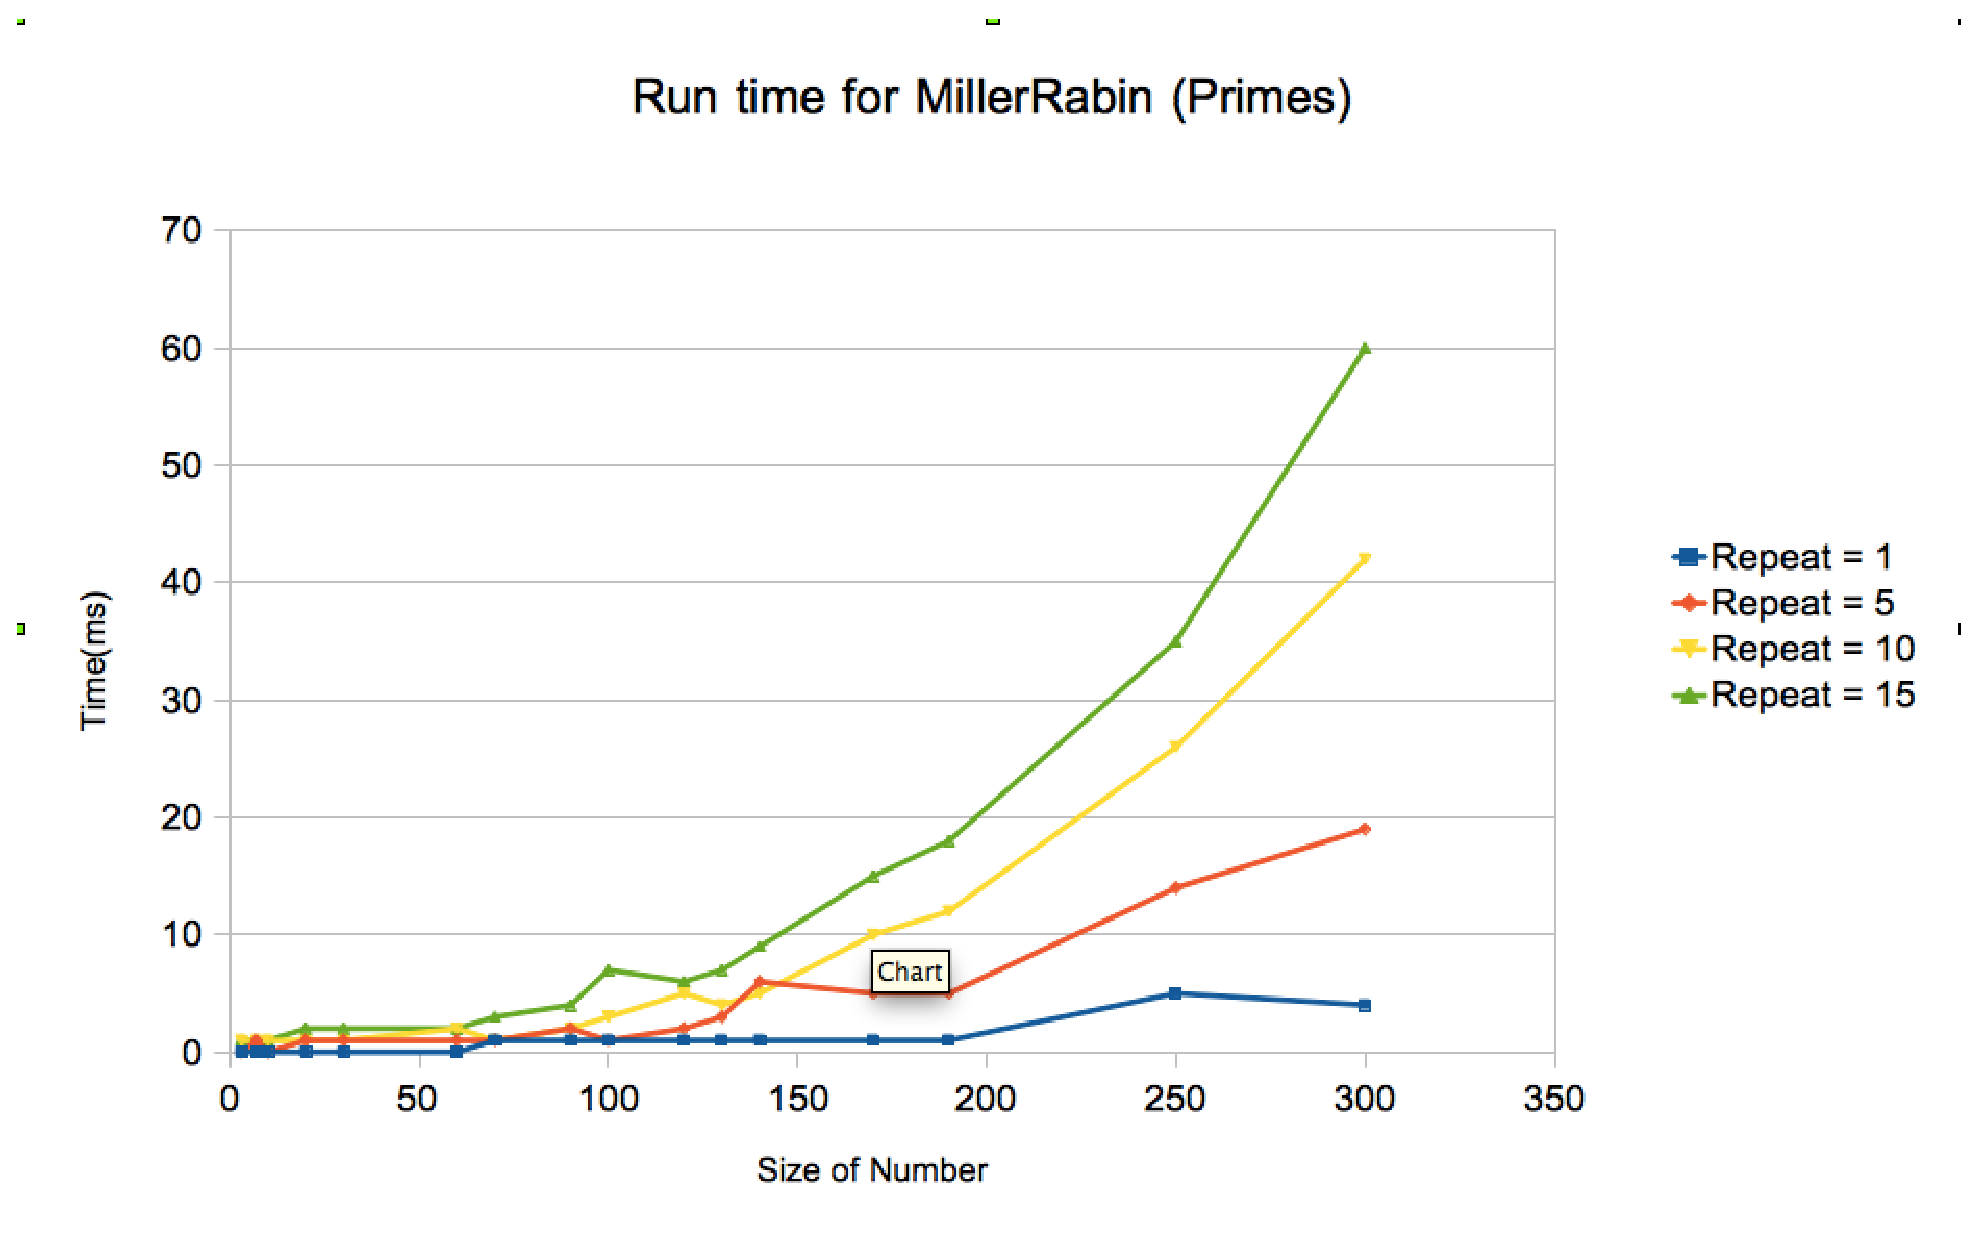
\includegraphics[scale=0.4]{./MR_P.eps}
\par\end{centering}

\caption{Runtime for Miller Rabin (prime)\label{fig:MR_P}}

\end{figure}
\begin{figure}[t]
\begin{centering}
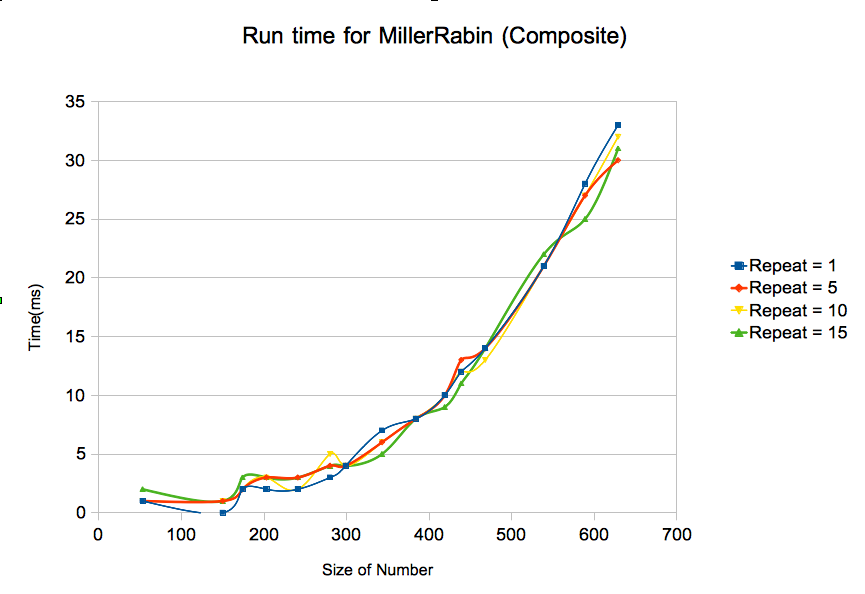
\includegraphics[scale=0.4]{./MR_C.png}
\par\end{centering}

\caption{Runtime for Miller Rabin (composite)\label{fig:MR_C}}

\end{figure}

\begin{figure}[t]
\begin{centering}
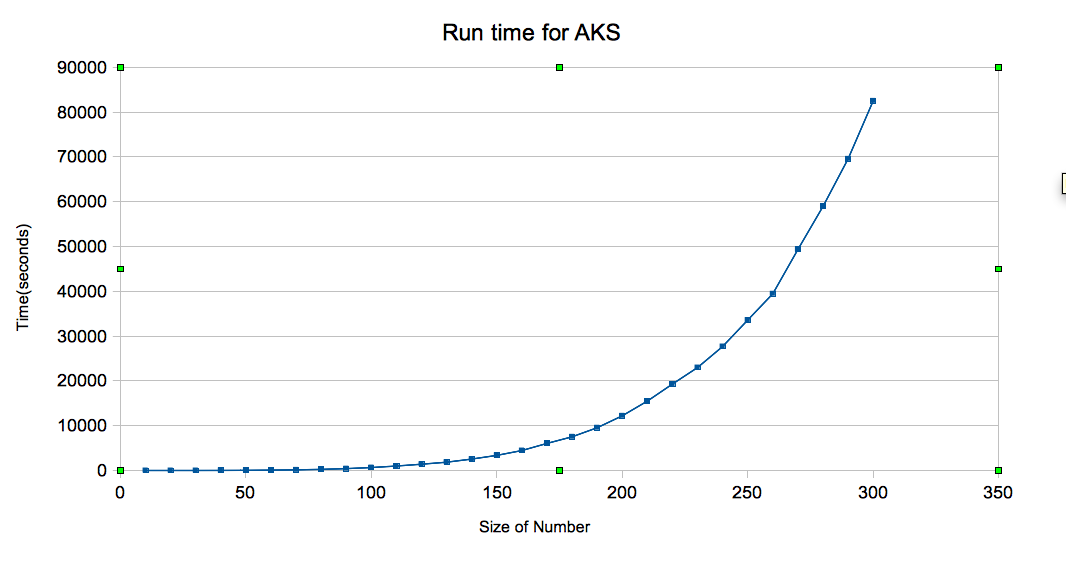
\includegraphics[scale=0.4]{./AKS.png}
\par\end{centering}

\caption{Runtime for AKS (our implementation)\label{fig:AKS}}

\end{figure}


\begin{figure}[t]
\begin{centering}
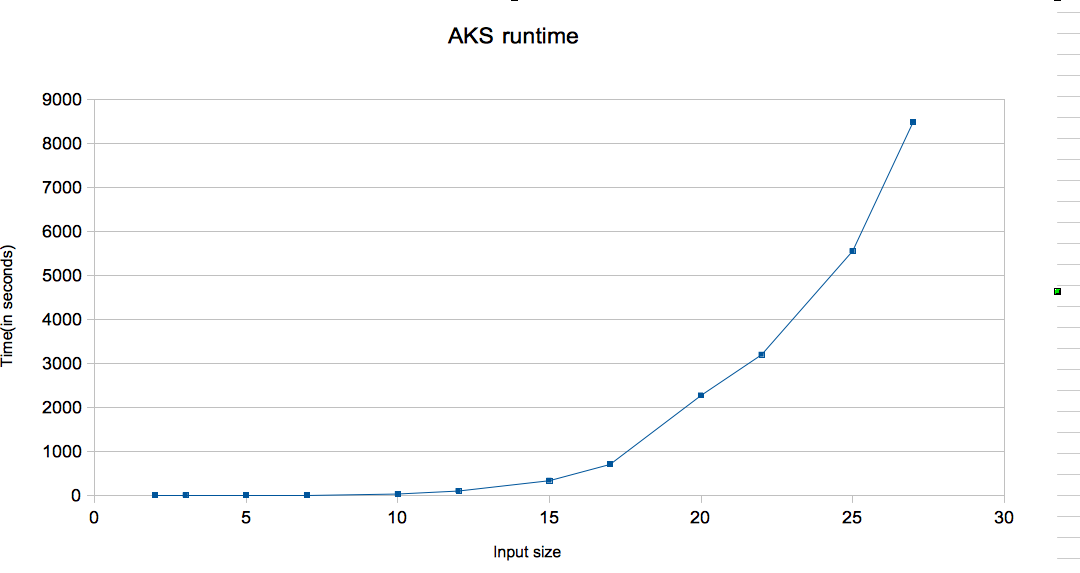
\includegraphics[scale=0.4]{./aks-ntl.png}
\par\end{centering}

\caption{Runtime for AKS (using NTL)\label{fig:AKS:NTL}}

\end{figure}

In this section we present the results of our implementation. We have experimented to large numbers (both prime and composites) and run both Miller-Rabin and AKS algorithms. In our implementation, we have used a  combined approach where we choose Miller-Rabin when the number is in such a range such that Miller-Rabin produces deterministic results. For numbers beyond that range, we the AKS algorithm. Our algorithm is disjoint depending on the input it receives. \\

Hence separate plots for AKS and Miller-Rabin Tests are presented here that captures the flavor of our algorithm. 
Since Miller-Rabin is a nondeterminisitc algorithm, we have experimented with extremely large primes and composite inputs separately to look out for any false positives. i.e. when a composite number is falsely reported prime. \\

In figure \ref{fig:MR_P} and figure \ref{fig:MR_C} presents the runtime for Miller-Rabin test for prime and composite numbers respectively. \\

The probability of reducing error in Miller-Rabin Test can be done by varying the number of iterations (values of $a$) that the test is preformed for every input. We have tried the number of iterations from the set (1, 5, 10, 15). And the result is presented. As expected, runtime increases as we increase the number of iterations. But still for all cases, the execution time is very small even for very large numbers. The maximum execution time that we obtain for a 300 digit number is of the order of ~ 60ms.\\

In figure \ref{fig:AKS}, we present the run time of the AKS algorithm that we implemented. As we see from the figure, the running time is very slow as the number of digits in the input increases. For an input of 300 digits, the AKS takes 80,000 seconds to converge. Even for inputs of smaller length the run time of AKS is orders of magnitude more than that of Miller-Rabin test. \\

In figure \ref{fig:AKS:NTL}, we present the results of the AKS implementation using the NTL and GMP libraries. As seen from the figure, this implementation is much slower and takes 8000 seconds for inputs as small as 30 digits in length. \\

So we see that our implementation using java and the BigInteger library is much more efficient as compared to the existing implementation in C++ using GMP and NTL libraries. \\

\textbf{Configuration of Machine used}\\
Processor: Intel Core i7 2.8 GHz\\
Memory: 4Gigabytes\\

\section{Conclusion}
In this project we have explored different methods for primality testing and tried to come up with an efficient  approach that can test for large primes. After exploring different avenues of the current state of the art of primality testing, we focused on mainly two different algorithms - Miller-Rabin which as a probabilistic algorithm and AKS which is the only polynomial time deterministic algorithm to test primality to date. Our experiments show that though AKS is deterministic and theoretically runs in polynomial time, for large numbers its execution time is painfully slow. Whereas, the non-deterministic Miller-Rabin algorithm executes very quickly for even large numbers. Though Miller-Rabin never tells a prime number as composite, it can give false positives,i.e. flag one composite number as prime. However, by adjusting the number of trials we can make the probability of false alarms negligibly small. In fact, for all the experiments we run we never encountered any false alarms. So, we believe that until and unless a complete deterministic primality testing is required , for all practical purposes one should use Miller Rabin test , adjusting the probability of false positive as required. It should be noted that, for numbers below certain range Miller Rabin test can be made fully deterministic. So though we have presented a combined approach of AKS and Miller-Rabin as a deterministic test for primality, we recommend that based on the application need one should try to use Miller-Rabin as much as possible.  
%\bibliography{report}
\newpage
\section{References}
$[1]$ - Agrawal, Kayal and Saxena. Primes is in p. Annals of Mathematics (2004), 781-- 793.\\
$[2]$ - Advanced Algorithms, University of Utah, Fall 2011. \url{https://learn-?? uu.uen.org/courses/48426/files/3870539/download?wrap=1.}\\
$[3]$ - \url{http://users.auth.gr/~karanika/Ergasies/string1.pdf}\\
$[4]$ - Wikipedia. Prime number. \url{http://en.wikipedia.org/wiki/Prime_number.}\\
$[5]$ - Crandall and Papadopoulos 2003\\
$[6]$ - \url{http://en.wikipedia.org/wiki/Miller%E2%80%93Rabin_primality_test}\\
$[7]$ - \url{http://en.wikipedia.org/wiki/AKS_primality_test}\\
$[8]$ - \url{http://en.wikipedia.org/wiki/Adleman-Pomerance-Rumely_primality_test}\\
$[9]$ - \url{http://en.wikipedia.org/wiki/Sieve_of_Eratosthenes}\\
$[10]$ - \url{http://www.math.twsu.edu/history/men/eratosthenes.html}\\
$[11]$ - \url{http://www.pballew.net/FermLit.html}\\
$[12]$ - \url{http://en.wikipedia.org/wiki/Fermat's_little_theorem}\\
$[13]$ - \url{http://en.wikipedia.org/wiki/Carmichael_number}\\
$[14]$ - \url{http://terrytao.wordpress.com/2009/08/11/the-aks-primality-test/}\\
$[15]$ - \url{http://en.wikipedia.org/wiki/P%C3%A9pin's_test}\\
$[16]$ - Abdullah Hosain, Implementation of the AKS Primality Testing Algorithm, December 2007.\\
$[17]$ - \url{http://en.literateprograms.org/Special:Downloadcode/Miller-Rabin_primality_test_%28Java%29}\\
$[18]$ -  Salembier and Southerington. An Implementation of AKS Primality Test. 2005.\\
$[19]$ - NTL: A library for doing Number Theory. \url{http://www.shoup.net/ntl/}\\
$[20]$ - The GNU Multi Precision Arithmetic Library. \url{http://gmplib.org/}\\


%%% End document
\end{document}
